\subsection{Features} \label{features}
This chapter details the different features that were implemented during the project. They are mostly language agnostic features that were implemented according to the language server protocol to offer a richer IDE experience. The backbone of the language server protocol is the interface IConnection. When the plugin is started, an instance of this interface is established which allows communication from the client (the IDE) to the server (the plugin / the language server). On this connection, generic requests and replies can be sent and received, but the language server protocol also offers defined messages for common IDE features. \newline
For instance, if the plugin wants to support rename element, it must provide a callback to the onRenameRequest on the connection. The input to this callback usually is the information needed to answer the request, typically a document and a position in it. The language server is then free in its implementation on how to answer these requests. \newline
Usually this is done by a so called provider, a class which implements at least one method that can answer such a request. This method is then registered as a callback to that element when the plugin is initialized.\newline
This project also chose this approach, for every IDE feature a provider was implemented, which carries out the task of answering such a request. The providers themselves are heavily based on the symbol service. Both the providers and the symbol service are explained below. 


\begin{figure}[H]
	\centering
	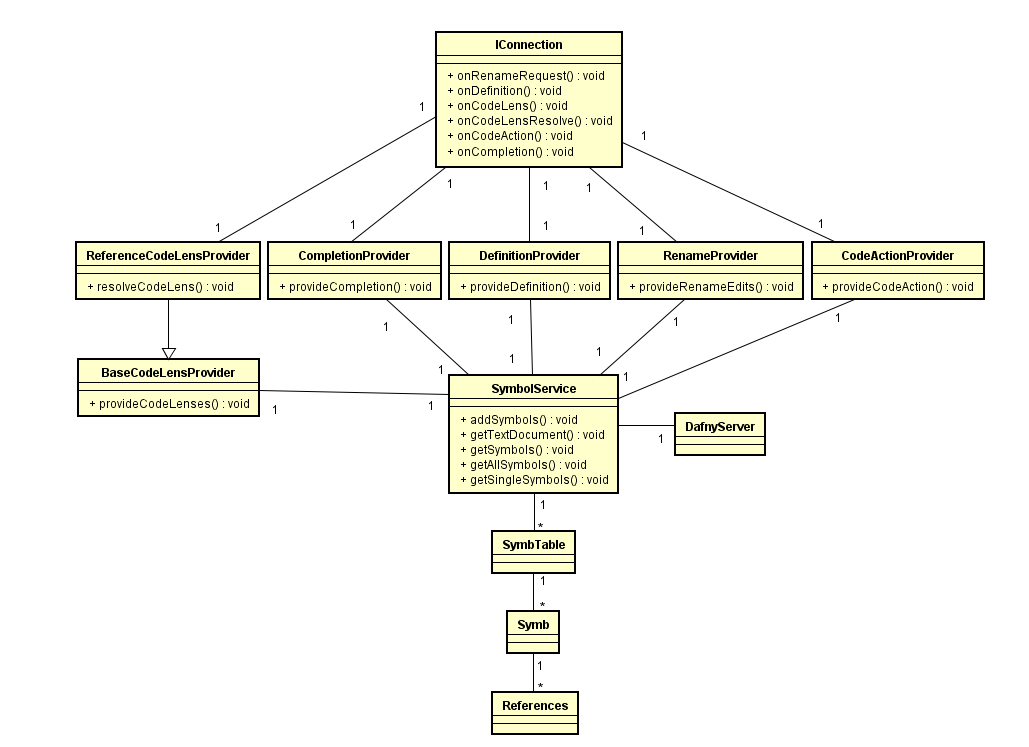
\includegraphics[width=1\textwidth]{img/featureArchitecture}
	\caption{How the IDE-features are integrated into the language server}
	\label{fig:featurearchitecture}
\end{figure}


\subsubsection{CodeLenses} \label{codelenses}
CodeLenses are Visual Studio Code a feature which is also common to many other IDEs. The idea is to display meta information about certain pieces of codes, for instance classes and methods. In Visual Studio Code this is done  by adding an additional line of text to the editor wherever a codeLense should  be placed. \newline

Since this can be used to quickly gain a deeper understanding of a code base, it was decided to integrate this feature. Another reason was that it is widespread in different IDEs, so that programmers have become accosted to it. \newline

\begin{figure}[H]
	\centering
	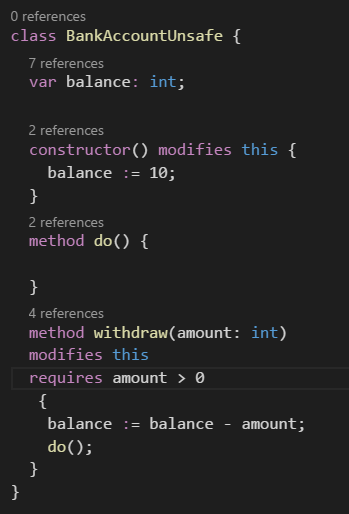
\includegraphics[width=0.5\textwidth]{img/codelensesClosed}
	\caption{Code Lenses used with Dafny}
	\label{fig:codelensesclosed}
\end{figure}

The first decision to be made was for which elements in the code codeLenses should be displayed. The trade off here is to  provide enough information to work comfortably with the code base and not to clutter the workspace with codeLenses It was decided to display codeLenses for classes, methods (including constructors) and fields, since they tend to have a wide scope in the code bases \newline

A second consideration was which information should be displayed in a codeLens. When codeLenses are language specific and do not for instance stem from a plugin which displays code metrics or similar, usually references and usages of the element are displayed. Since this allows the programmer to gain a deeper understanding of control flow and regions affected by refactoring, it was decided to display this information also for the Dafny plugin. CodeLenses also allow commands to be executed when clicked upon, a logical conclusion is to implement go to reference when a reference in a codeLens is clicked.\newline
Since the tasks of finding the elements which need a codeLens and constructing the codelens itself are very different, the implementations were separated in a base class and a child class. The base class answers the onCodeLens request of the connection and the child class then answers the onCodeLensResolve request. The reasoning for this lies in possible future expansion, as maybe additional information should be displayed in a codeLens. This can be done in an own child class, the produced codeLenses (which stem from the same placeholder codeLens) then are automatically merged by Visual Studio Code. This design was also inspired by the GoLang Plugin. 

\begin{figure}[H]
	\centering
	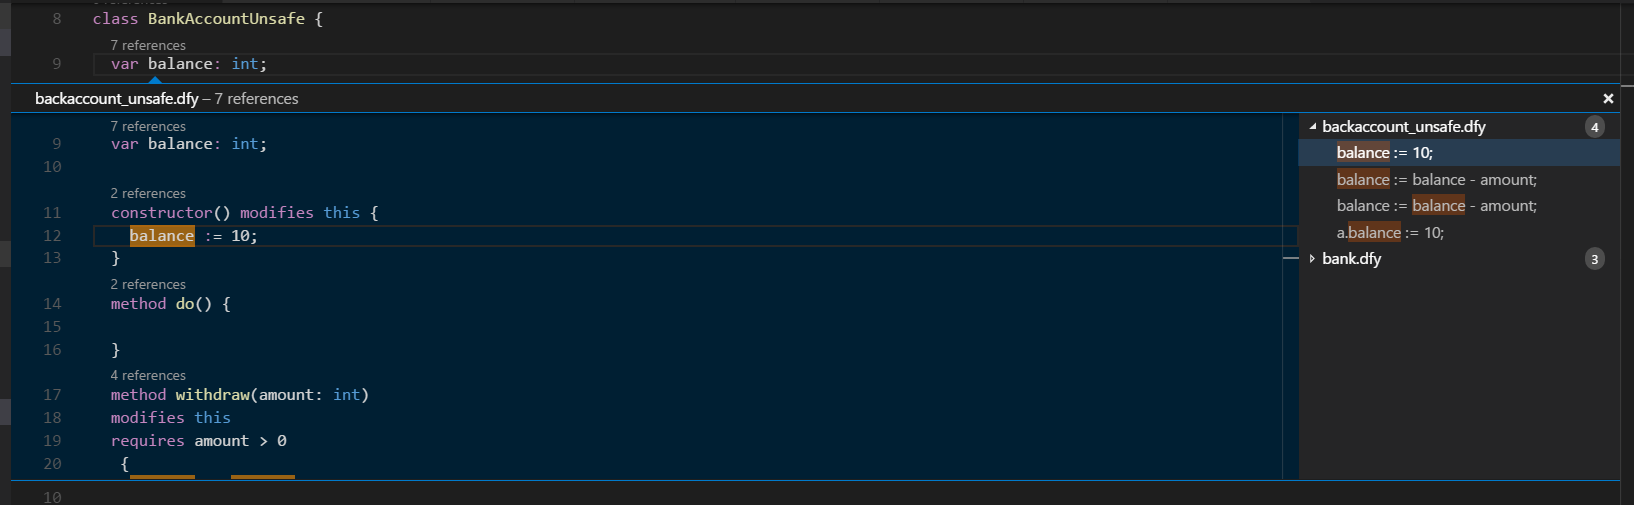
\includegraphics[width=1\textwidth]{img/codelensesExpanded}
	\caption{Expanded codeLens showing the references to the field balance}
	\label{fig:codelensesexpanded}
\end{figure}

The only challenging aspect when implementing this feature is that references can't be determined via a simple text search, since different classes could have members with the same name. To only display unambiguous references, the search has to be done via the fully qualified domain name of the symbol. Since information about references is needed often, all references are determined by the DafnyServer and returned together with the symbol information to the symbol service. This allows for simple processing in the language server itself and the references are updated in real time, since the symbol service refreshes the symbols for a file when it is changed. Off course also the file path belonging to the file in which the reference occurs is returned by the symbol service. This is needed when a reference is a file external to the defining one and the go to reference command is invoked.\newline
When given locations of the references, it is possible to let Visual Studio Code highlight them in the preview window which opens when a codeLens is expanded. Visual Studio Code also groups references according to the file path in the location, so the programmer gets to see a map of all references ordered by containing file to the right of the preview window and can quickly navigate to them.

 \subsubsection{Code Completion} \label{codecompletion}
 Code completion has become a standard feature for IDEs. Microsoft calls it IntelliSense in its products. It enables programmers to rapidly write code without having to keep all definitions in mind. Usually, when the programmer starts typing, a little popup appears in which the programmer can choose options that complete the code he is currently writing. \newline
 
 Since this is arguably one of the most helpful features in IDEs, the implementation thereof was paramount to the completion of this project. \newline
 
 \begin{figure}[H]
 	\centering
 	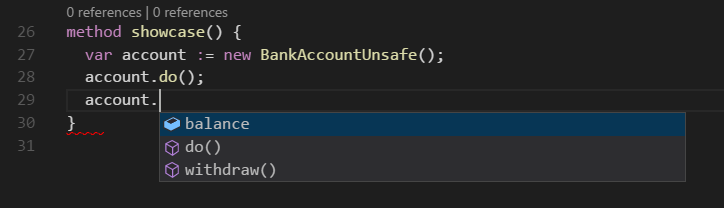
\includegraphics[width=1\textwidth]{img/codeCompletionOverview}
 	\caption{Popup with completion options}
 	\label{fig:codecompletionoverview}
 \end{figure}
 
 There are several different considerations when implementing code completion in a language server. The first one is to define which typed characters should trigger a completion request. Ideally, an IDE supports the programmer with completion regardless of the current context. Next to performance, another reason to narrow down the trigger selection is that not all contexts warrant meaningful suggestions for completion. In this project, a pragmatic approach was chosen where completion is triggered when ever a "." is typed, a situation where the programmer usually wants to access a member of an element. Since there is usually a designator present before the ".", there is also enough knowledge present about the current context to offer meaningful options. \newline
 In order to support this, the symbol service stores all variable declarations so the plugin knows about the type of all expressions that can be followed by a ".". The completion request comes with a position in the current file as an argument, so the first task is to resolve the expression and find out the fully qualified name of each element. The language server then searches the symbol service for all members that are defined in the class with that fully qualified name and sends them back as completion suggestions. \newline
 Visual Studio Code then handles all further actions, for instance, once the popup is displayed and the programmer continues to type, it removes all suggestions that don't start with the typed characters. It is also possible to display further information regarding the suggestions. The plugin already details if the completion is a field or a method, which Visual Studio Code provides  separate icons for. When the suggestion is a method, the preconditions, if any, are also displayed, so the programmer already knows the constraints he is writing under. \newline
 
 \begin{figure}[H]
	\centering
	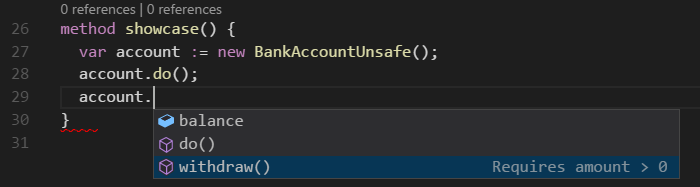
\includegraphics[width=1\textwidth]{img/codeCompletionMethod}
	\caption{Suggestion displaying precondition}
	\label{fig:codecompletionmethod}
\end{figure}

The implementation is straightforward, as the symbol service already provides ways to resolve the fully qualified name of an expression and if it as an alias for an element of a class, all therein defined methods and fields can simply be collected. The method and field symbols in the symbol services also contain all additional information which is displayed in the popup. Possible improvements in the completion feature would be support of built in methods and functions and also offer context aware completion when the programmer starts to type an identifier. 

\subsubsection{Go to Definition} \label{gotodefinition}
Another common feature in modern IDEs is go to definition. It enables the programmer to quickly jump to the definition of a code element he is currently working with in order to gain further insight about it. This can usually be done either via a hot key for the current cursor position or an option when opening the context menu via a right click, Visual Studio Code offers both ways.\newline
Since, similar to codeLenses, this is a feature which is elemental to all modern IDEs and provides great overview over a project, the implementation of this feature had a high priority in this project. \newline
 \begin{figure}[H]
	\centering
	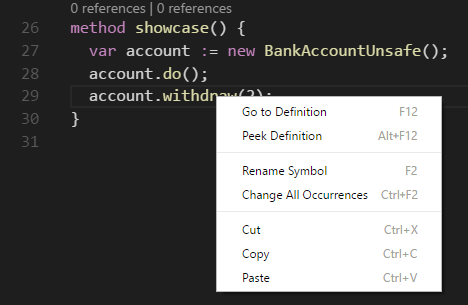
\includegraphics[width=0.5\textwidth]{img/goToDefinition}
	\caption{The Definition Features}
	\label{fig:gotodefinition}
\end{figure}
The language server protocol offers an on definition request, which has the URI of the file and the position for which a definition is requested as parameters. The plugin then first tries to resolve the word at the position which could lead to a definition. When a word could be resolved, the plugin tries to determine if the expression is an alias for an element of a class or if it stands for an access of a member of one. If this is the case, the fully qualified name of the symbol can be determined via the symbol service, as it stores information about all definitions and declarations. The plugin than finds the unambiguous definition via the fully qualified name and responds with the location of that definition. This also works if the definition is in an external file in the same workspace. \newline
If, for whatever reason, the fully qualified name cannot be determined, the plugin tries to match the selected word with any symbol cached in the symbol service. This approach only works as best effort though, as different classes could defines methods with the same name for example. If no match is found at all, no definition is provided. \newline
Visual Studio Code offers two options when searching for definitions, either go to definition which immediately opens the returned location in an editor or peek definition, which shows the definition in a little popup. \newline
 \begin{figure}[H]
	\centering
	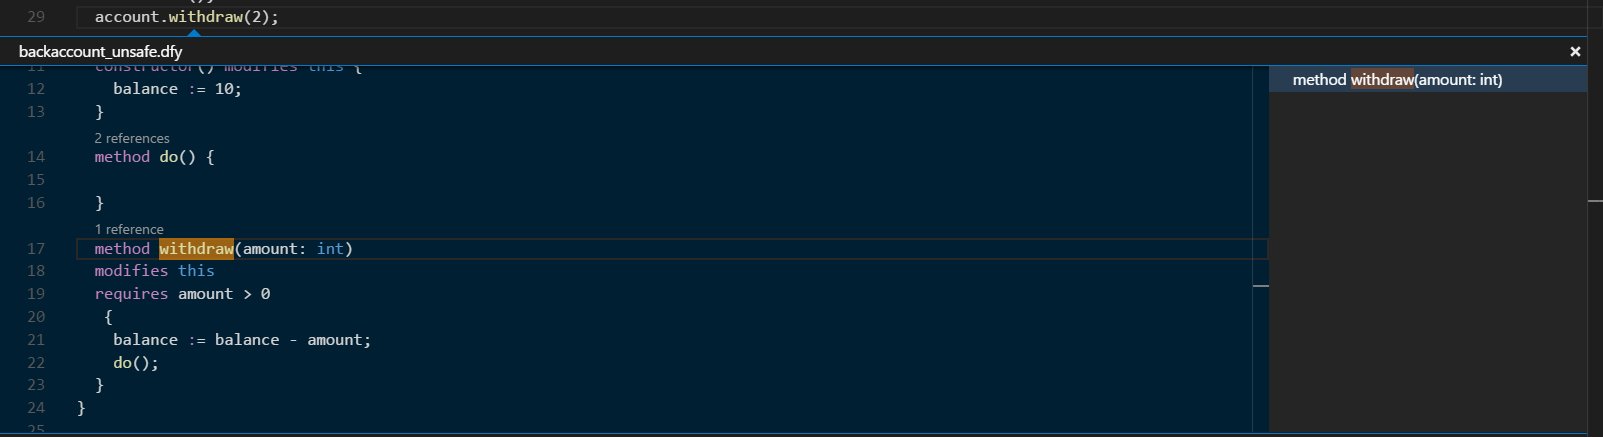
\includegraphics[width=1\textwidth]{img/goToDefinitionPeek}
	\caption{Overlay of peeked definition}
	\label{fig:gotodefinitionpeek}
\end{figure}
Extensions to this feature could be a context aware heuristic when a fully qualified name cannot be determined where for instance the current and nearby files are preferred when searching for definitions. Also, when polymorphism comes into play and the actual implementation cannot be determined, at the current state the first possibility is returned. The could be enhanced by offering all possible definitions.


\subsubsection{Rename Element} \label{renameelement}
Rename element is a feature essential to refactoring. It is widespread in IDEs and allows to quickly make code better readable. Visual Studio Code offers built in support for renaming either via a hot key or the context menu. \newline
Because of its importance in refactoring, which is one of the most important tasks when programming, implementing this feature belongs to the core scope of this project. \newline
The language server protocol, as with many other features, offers a request for renaming with the URI of the file in which the command was invoked and the position belonging to the command. Additionally, the new name of the element should have is also given as an argument. The protocol expects a collection of textedit commands, which entail an URI of file, and ranges in that file which should be replaced with a word. \newline
As often with the language server protocol, the first step when implementing the feature is to determine the element at the position which is given as an argument. When the position can be resolved to a meaningful word, the plugin tries to determine if it is either an alias for an element of a class, or a member of class, for instance a field or a method. If it can do so with absolutely certainty, the fully qualified name of that element is obtained. The next step is trivial, since the symbol service already caches all references to a symbol, information which it gained through the DafnyServer. The plugin can simply build textedits out of all references, since the reference already contain all necessary information such as the containing file and their position therein. This therefor also works across multiple files which reference the same element, as long they are open in the same workspace. Those textedits are then returned from the language server to Visual Studio Code, which does all the actual replacing. \newline
  \begin{figure}[H]
 	\centering
 	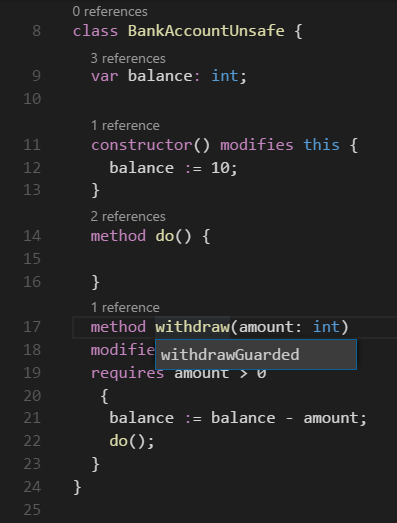
\includegraphics[width=0.5\textwidth]{img/rename}
 	\caption{Renaming an element in Visual Studio Code}
 	\label{fig:rename}
 \end{figure}
Since this feature actually changes code that is worked with, the implementation must be very robust and failsafe. Thus, it was implemented very defensive. It the location of a requested renaming cannot be resolved to a meaningful word, the request is ended without dictating any changes. The same holds if a word can resolved, but it cannot be matched to a fully qualified name. In this case, possible references could be ambiguous, so no action should be taken. To further limit the possibility for failure, the scope for this feature is very small. The current implementation only allows for renaming of class members such as fields and methods, since these can be resolved with absolute certainty.\newline
When extending this feature, it would be beneficial to also be able to rename local variables for instance. To do this, the symbol information which the DafnyServer returns to the symbol service would have to be enriched with detailed scope information to allow being able to exactly say which regions are prone to renamings and which are not. 

\subsubsection{Quick Fixes} \label{quickfixes}
Quick Fixes are a versatile feature in IDEs which basically allow to do any manipulation to code. Usually they are offered as reactions to diagnostics which were provided earlier. A simple example would be implementing a spell checker this way, offering to replace a wrongly written word with the correct spelling. \newline
Since this feature has no clear implementation guideline, and the plugin designer can implement almost anything that he likes this way, this was an obvious place to implement Dafny specific feature in the plugin. A deeper insight why the following features were chosen can be found in \ref{addCodeActions}. \newline
They way this works in Visual Studio Code is that when the diagnostic stage for the file has been completed, where all things such as compiler warnings or custom warnings are generated, a new request is fired at the language server. This request holds a collection of all diagnostics on the current file and the the language server is free to either do nothing are provide commands for some diagnostics in the collection which often aim to resolve the shortcomings detailed by the diagnostic. \newline
  \begin{figure}[H]
	\centering
	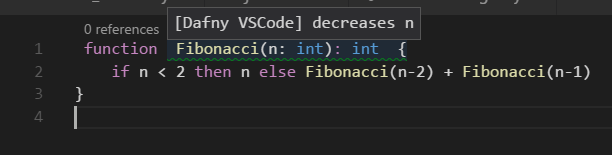
\includegraphics[width=0.7\textwidth]{img/diagnostic}
	\caption{Visual Studio Code displays a diagnostic}
	\label{fig:diagnostic}
\end{figure}
The current stand of the projects offers three code fixes to resolve Dafny specific diagnostics. \newline
The first one is a common situation where a programmer fails to capture his intention that an expression should either decrease or increase when working with recursion or loops. It can also be the case that an expression must always evaluate into a certain range, this is for instance the case when an expression that is used as an index to an array is not constant within a loop. The remedy is simple, a decrease / increase guard with the expression in question must be added at the correct location. In case an expression must be within a certain range, the same intent can be written as an invariant. \newline
  \begin{figure}[H]
	\centering
	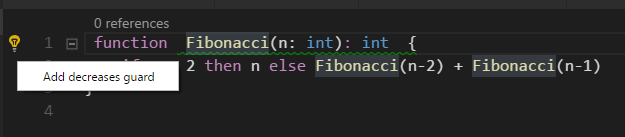
\includegraphics[width=0.7\textwidth]{img/decreaseGuard}
	\caption{Offering a code fix to add a guard}
	\label{fig:decreaseguard}
\end{figure}
This situation can easily be identified through the message within the diagnostic, since Dafny always gives this message in the same format. The expression that has to be decreased can also easily be parsed out of this message. The placement of the guard is a little more difficult, the implementation tries to find the first block in which the variable is not in scope anymore. The guard is then inserted before the block containing the first usage. \newline
  \begin{figure}[H]
	\centering
	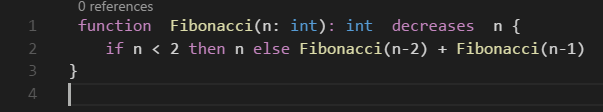
\includegraphics[width=0.7\textwidth]{img/decreaseGuardApplied}
	\caption{Program after the code fix}
	\label{fig:decreaseguardapplied}
\end{figure}
The second code fix the plugin offers is very similar, but this time the constraint is that an object may be null when it should not. The situation again is easily detected through the message in the diagnostic, and also the expression which should not be null can be parsed through it.
  \begin{figure}[H]
	\centering
	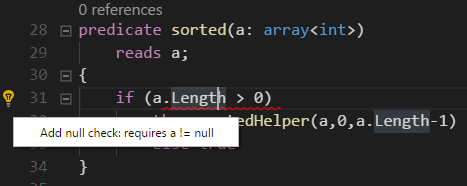
\includegraphics[width=0.7\textwidth]{img/nullCheck}
	\caption{It should be made sure that an element is not null}
	\label{fig:nullcheck}
\end{figure}
Also the search for the insertion position works very similarly. It then inserts the constraint in form of a precondition to the surrounding element. \newline
  \begin{figure}[H]
	\centering
	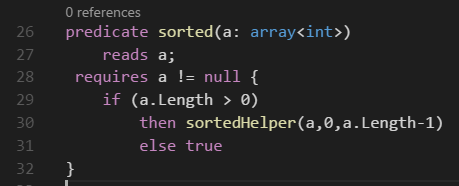
\includegraphics[width=0.7\textwidth]{img/nullCheckApplied}
	\caption{The precondition has been added}
	\label{fig:nullcheckapplied}
\end{figure}
The third code fix is to implement bound checking for expression which are used to index an array. This can either take the form of a precondition, if the expression is constant within the block of code in question, are the form of an invariant if the expression is dynamic (for instance in a loop).
The remedy is to apply the bound checking either through preconditions or invariants, depending on the context.
  \begin{figure}[H]
	\centering
	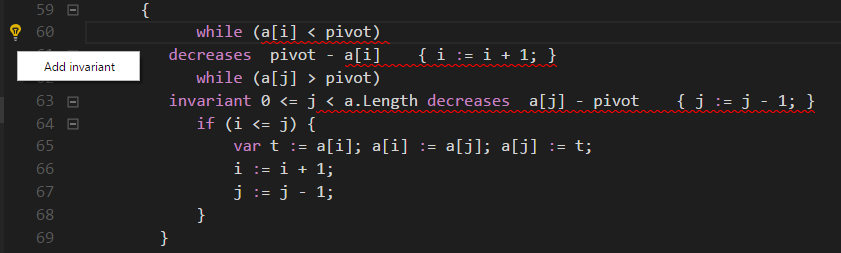
\includegraphics[width=1\textwidth]{img/indexOutRangeDiag}
	\caption{The expression may be out of range}
	\label{fig:indexOutOfRange}
\end{figure}
The first difficult part is to find the expression that is used as an index, as well as the identifier which stands for the array. Both is done through pattern matching on the code file in regard to the position of the diagnostic. Next it must be decided if preconditions or invariants should get generated, for this there must be knowledge about the context, e.g. if the expression is static through in the current block. This is done via the information saved in the symbol service and also some pattern matching. \newline
Finally, the invariant or the preconditions must be inserted into the correct place. For this, all identifiers used in the expressions must be matched against their declaration, in order place the guards when already all symbols are declared. \newline
  \begin{figure}[H]
	\centering
	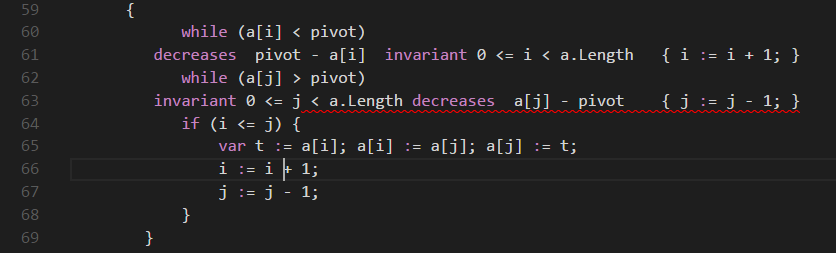
\includegraphics[width=1\textwidth]{img/indexChecked}
	\caption{Invariants for the loop were generated}
	\label{fig:indexInBound}
\end{figure}
At the current stand, only these three code fixes are implemented, the possible extensions are legion. One idea is to insert code that decreases a given expression when Dafny can't prove that an expression always decreases in a block were such a decrease clause was declared.\newline


\subsubsection{Counter Examples}
A useful features which also can provide a huge benefit, is to show an example which violates the contract, if the program can't be verified. Especially if the method is large with many branches, it can be very difficult to see how an example could look like, which is not correct regarding the contract. \newline
Z3 verifies mathematical expression by trying to find a proof for the negation of the proof. That means if it finds a proof the program is not correct. But more important Z3 finds a assignment for the different variables which violates the contract. This knowledge can be used to show a counterexample in Visual Studio Code. The only big step is to translate the counterexample, which is called model in Z3, back into something that can be matched with the Dafny program. Fortunately this is already done in the DafnyProvider in Boogie. Additionally to get only the necessary information out of it and also to show the values of class fields the translation needed to be extended. At the end a new verb counterExample was introduced, which returns a counter example json encoded. Thereby it was possible to show assignments of the variables on each line in Visual Studio Code. \newline
This is a easy example of a invalid method which should return the ABS, but misses to handle negative numbers correctly. 
\begin{figure}[H]
	\centering
	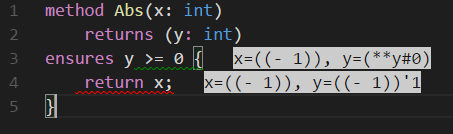
\includegraphics[width=1\textwidth]{img/counterModel}
	\caption{CounterExample is shown in Visual Studio Code}
	\label{fig:counterModel}
\end{figure}

Below is a more complex example of a class. The goal of the withdraw method is to prevent the balance to be below zero. Therefore the postcondition "ensures balance >= 0" exists. With help of the countermodel it becomes clear, that the amount is to big. It is bigger than zero though, but this precondition is wrong. It should be that the balance must be smaller than balance. On the first line it shows, that the balance is 2275 and the amount 2276. This results that the balance is after the subtraction negative. 
\begin{figure}[H]
	\centering
	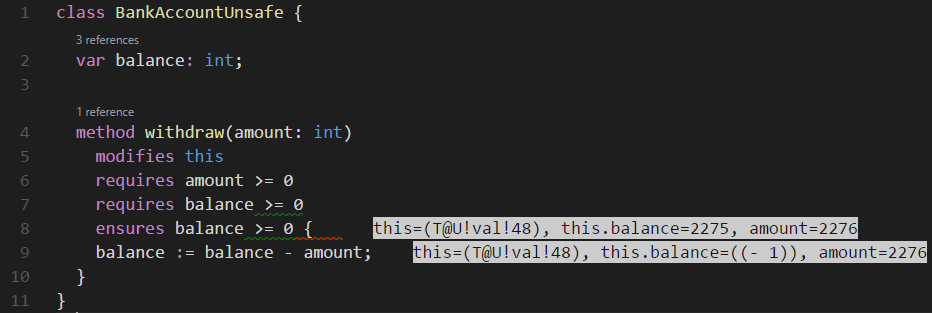
\includegraphics[width=1\textwidth]{img/counterModelBank}
	\caption{CounterExample inside a class}
	\label{fig:counterModelBank}
\end{figure}
